This chapter will go into the structural nature and coming together of this thesis project. The chapter starts by introducing Research through Design, as presented by Christopher Frayling before we go into the practicalities of the project. Then we will list and give an overview of the activities conducted before we look at the project and discuss the design process against \autocite{zimmerman_research_2014}'s five steps to carry out an RTD project. Finally, the chapter is rounded off by discussing how knowledge has been generated through analysis of installation designs and showcasing how the research question has evolved throughout the project based on theoretical and analytical findings.

\section{Research through Design}
This thesis follows an approach to research practise called Research through Design (RtD). This research approach was first coined by \autocite{frayling_1994}, in a highly influential paper where he addressed the debate and confusion at the time around what research \emph{is}, what it \emph{involves}, and what it \emph{delivers}. Frayling critiques the stereotypical perceived difference between the Research field and the Art and Design field - whereas 'researching' stereotypically is seen as a cognitive practise, while art and design is seen as an expressive practise \autocite[p. 5]{frayling_1994}. Concluding that since many of the motivations and practises of the two fields are alike, there is a more productive distinction of the relations between research, art and design \autocite[p. 5]{frayling_1994}, namely: research \emph{into} art and design, research \emph{through} art and design, and research \emph{for} art and design.

According to Frayling, Research \emph{into} art and design is concerned with historical research, aesthetic and perceptual research, and research into theoretical perspectives on art and design \autocite[p. 5]{frayling_1994}. Research \emph{for} art and design on the other hand is research "where the end product is an artefact - where the thinking is, so to speak, \emph{embodied in the artefact}, where the goal is not communicable knowledge in the sense of verbal communication, but in the sense of visual or iconic or imagistic communication"\autocite[p. 5]{frayling_1994}. Lastly, Research \emph{through} art and design is concerned with either/ or materials research, development work (i.e. customising a piece of technology to do something no-one had considered before, and communicate the results), as well as action research (i.e. where a research diary tells, in a step-by-step way, of the experiment and result), underlining how "both the diary and the report are there to \emph{communicate the results}, which is what separates \emph{research} from the gathering of reference materials" \autocite[p. 5]{frayling_1994}.
\par

\section{Joint forces with two research buddies}
This thesis is based on extensive fieldwork and design activities that have been made possible because of a joint effort with two other master's students, Janni Rasmussen and Anh Thy Sandra Nguyen. In this thesis, they are referred to as research buddies. We all chose the same thesis outline but wrote separately and have developed different research agendas. In the early stages, we worked together to get to know the domain and context, for the most part discussing and sharing literature insights. Already, during spring 2021, we started to single out different areas of interest. Regardless of that, we have conducted almost all fieldwork together, yet with separate data-gathering guides and analyses.

\begin{figure}[H]
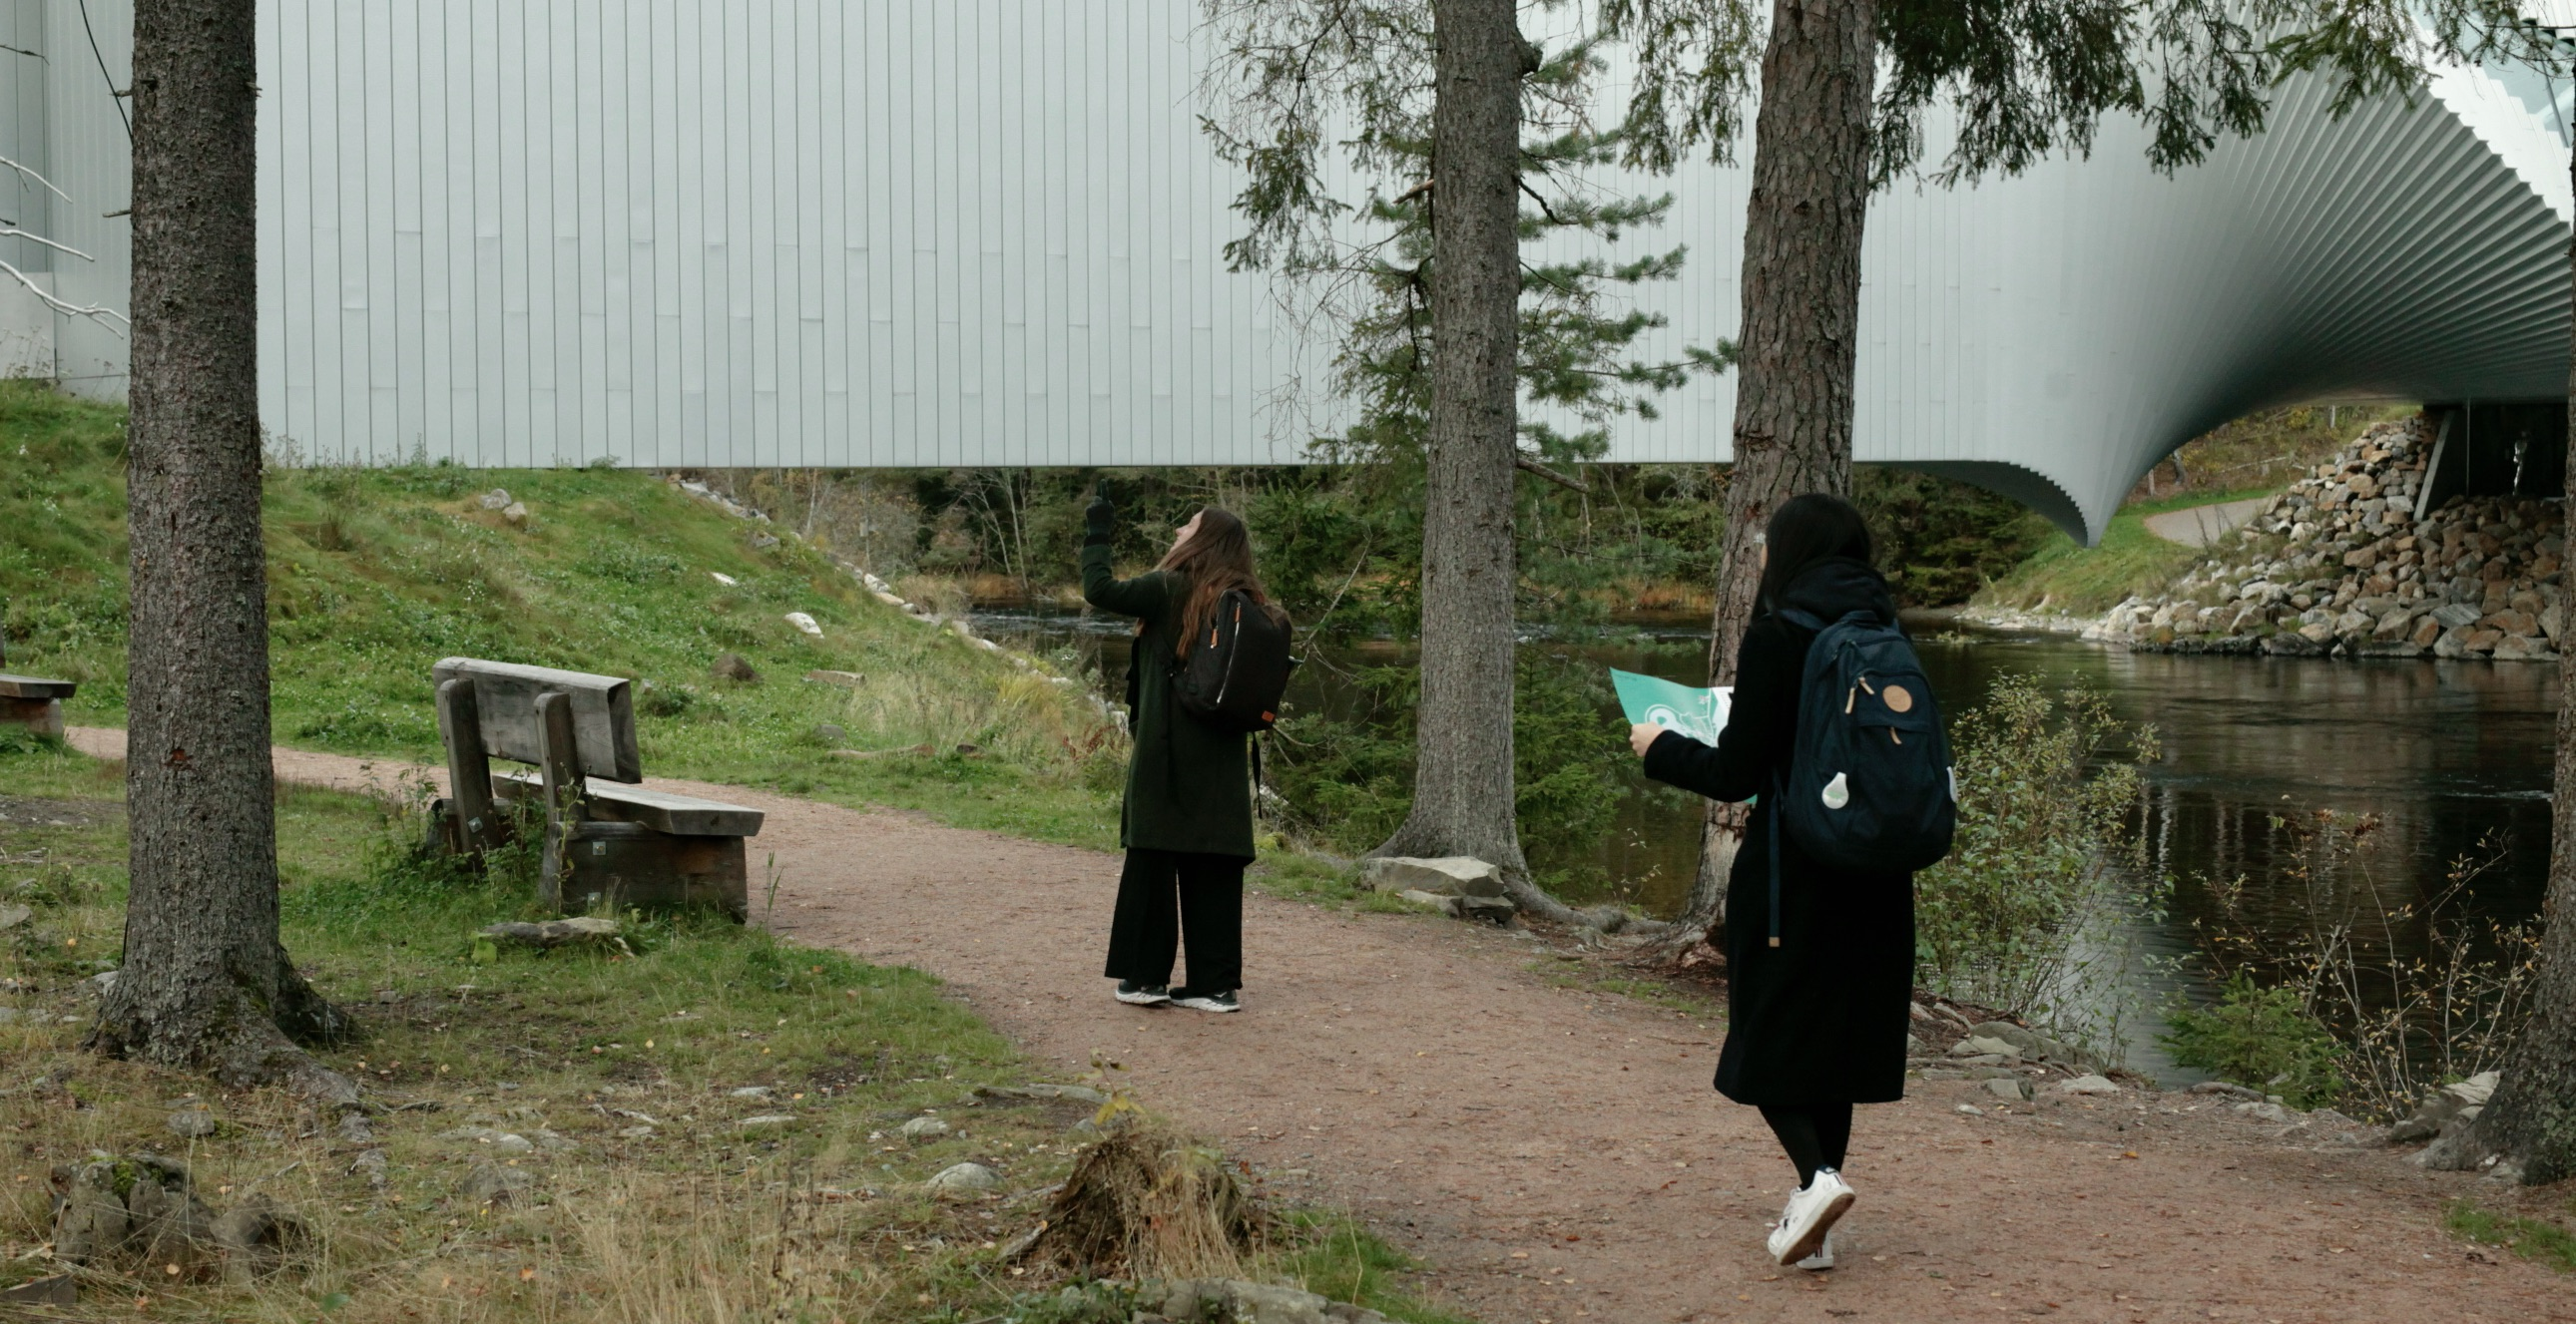
\includegraphics[width=12cm]{pictures/methodology/buddies.JPG}
\caption{The research buddies}
\centering 
\end{figure}

Janni is writing about engaging experiences with interactive installations in museums and exhibition spaces and how engagement can be facilitated with Tangible Interaction. In Sandra's study, she looks into how visitor engagement can be increased through narrative exhibitions and proposes principles for creating engaging, interactive installations in exhibition spaces.


\section{Collaborating with Klimahuset}
The original thesis outline was angled more practical; \emph{interactive and visual installations addressing sustainability}, and called for a collaboration with a museum addressing sustainability issues. Klimahuset is one of the University of Oslo's Natural History Museums. The museum is located in the Botanical Garden at Tøyen, Oslo, newly opened in 2019. Klimahuset represents the type of space where discourses on sustainability matters can be available to citizens as a museum. The museums aim to be open and accessible to all age groups, but they have particularly aimed to engage young boys aged 14-16. Through the university partnership, Klimahuset can provide access to museum staff, Docents, and visitors and an auditorium suited for exhibitions or workshops. Klimahuset has proven to be suitable for investigating a museum's agenda and discourse; the climate crisis. This provides the opportunity to investigate exhibition practices addressing sustainability issues such as Earth’s climate systems, consequences of global warming, solutions, and what actions individuals can do to contribute to a sustainable transition and future. 

\begin{figure}[H]
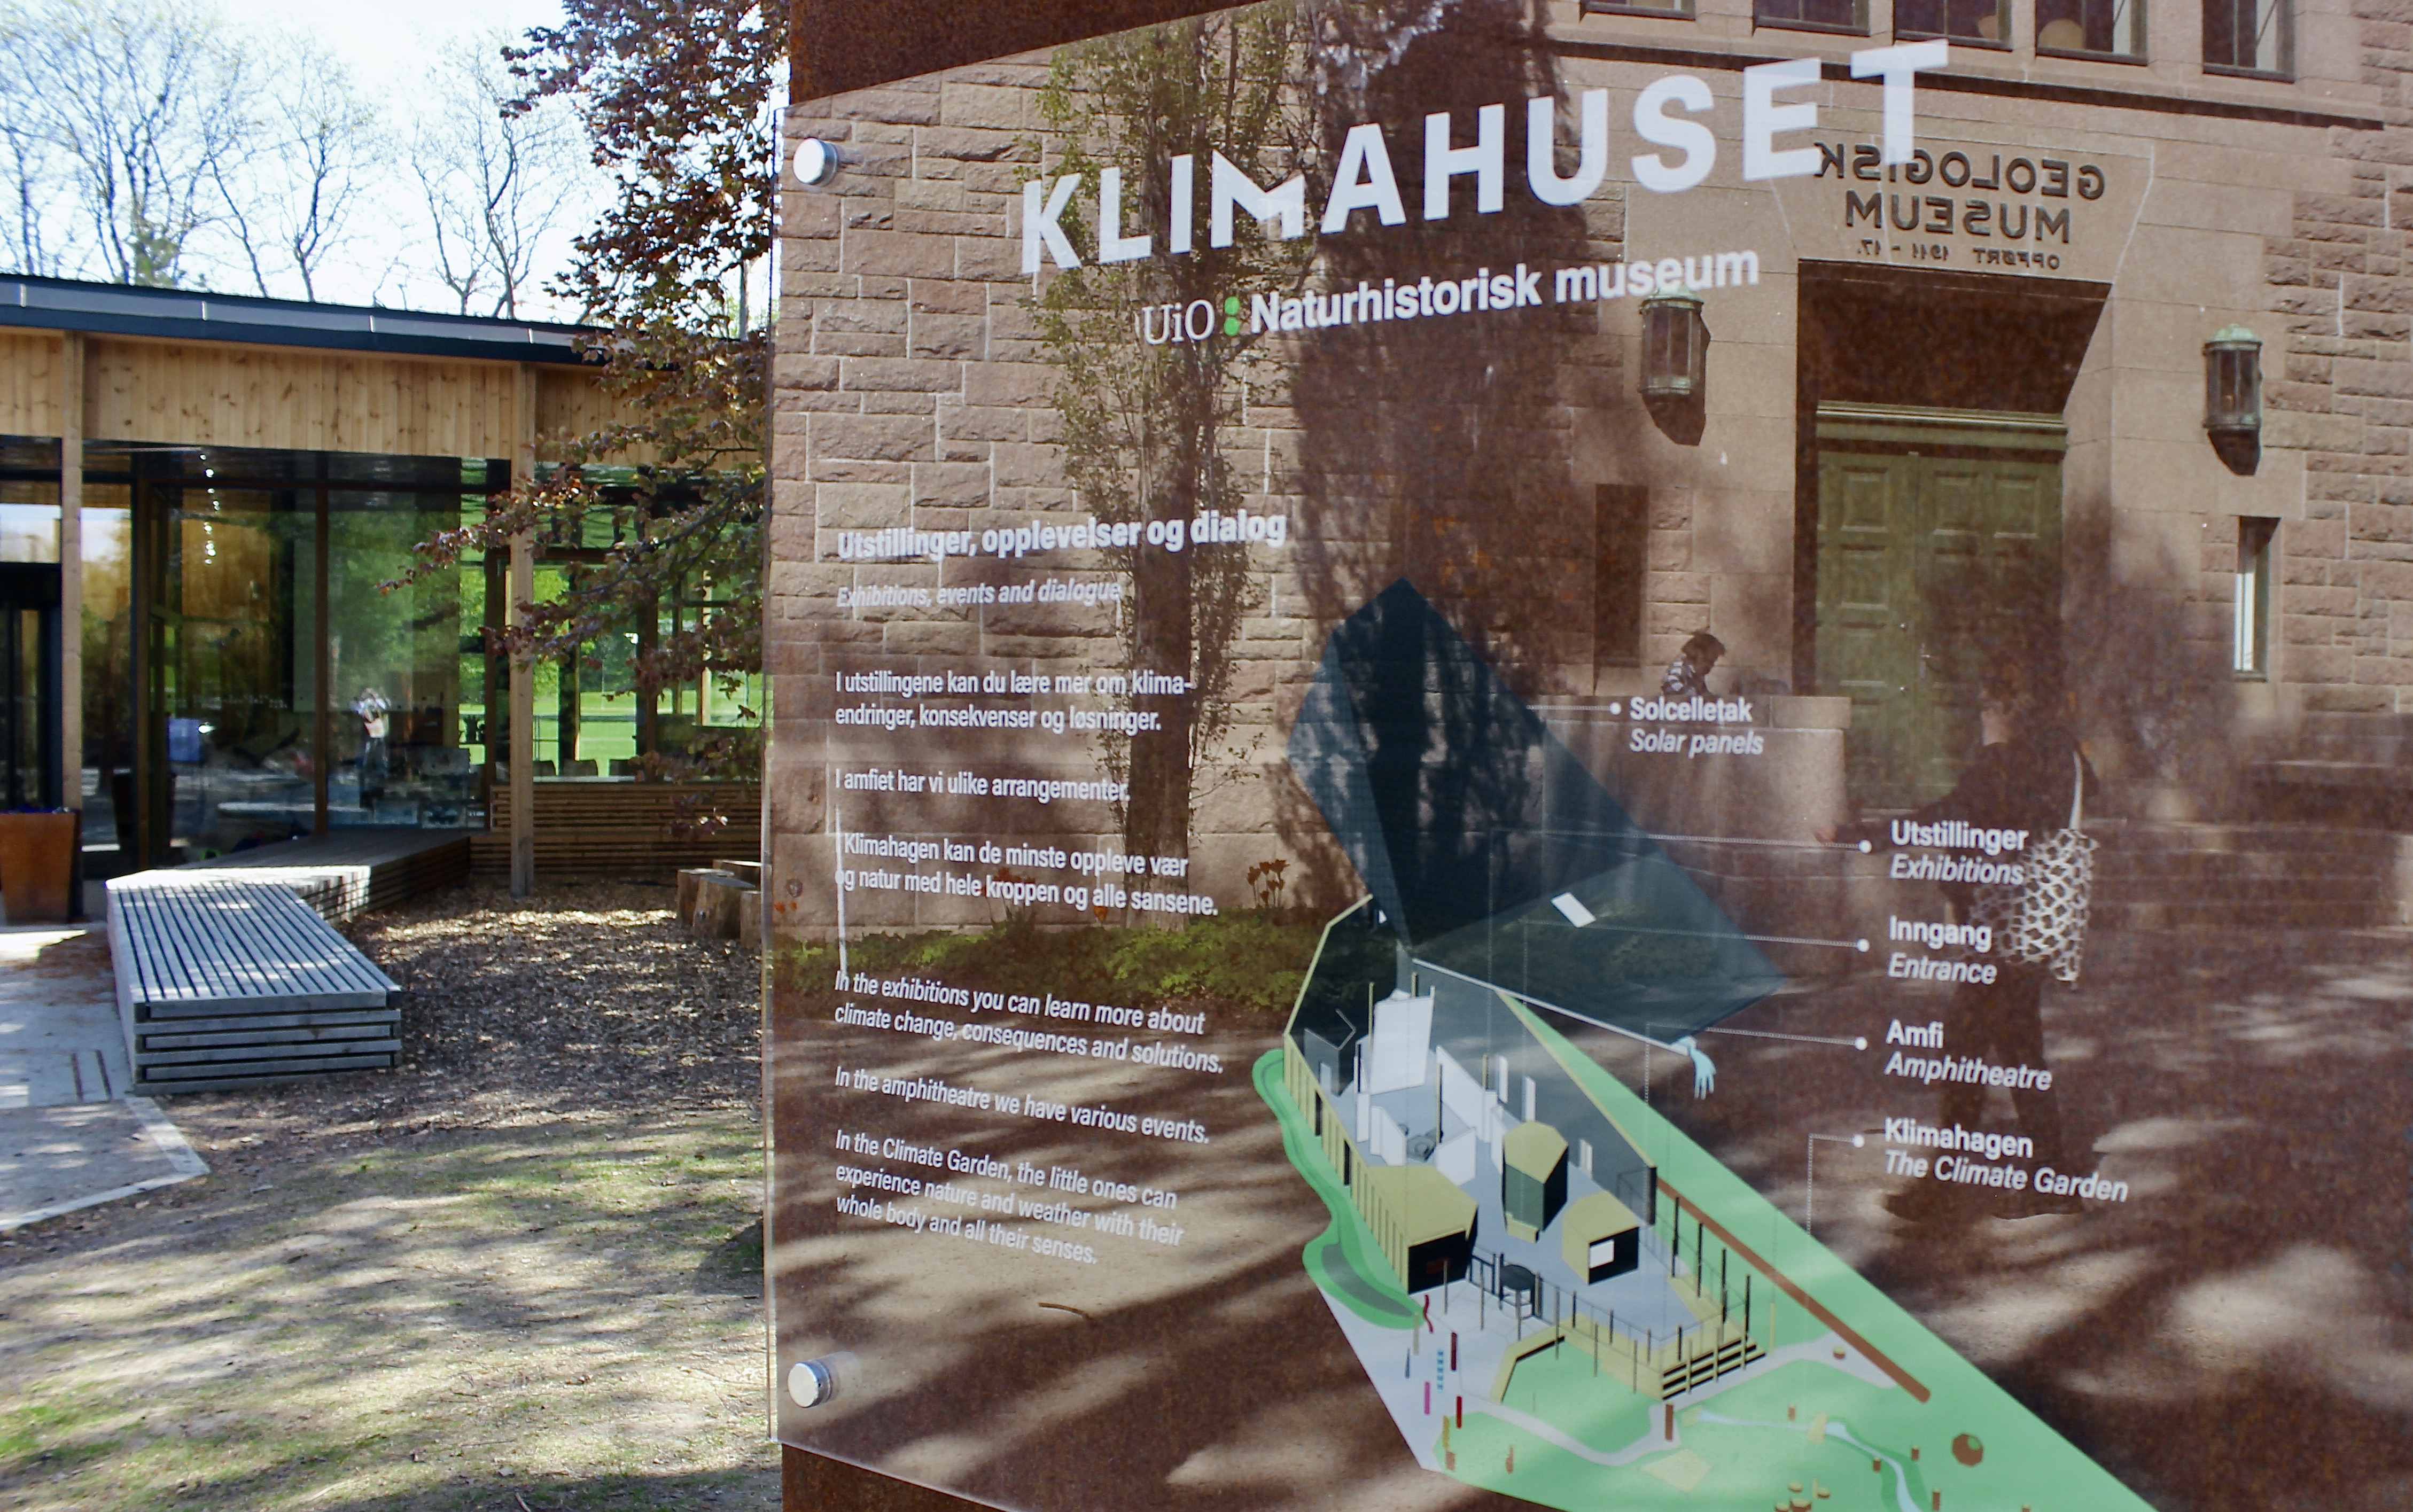
\includegraphics[width=12cm]{pictures/klimahuset/klimahuset_info.JPG}
\caption{Klimahuset entrance area}
\centering 
\end{figure}

\section{Timeline of events}
This section will account for the project timeline, presenting an overview and listing all the events that make up the project. Together with the research buddies, we conducted all the fieldwork together. Details on each event will be provided in chapter 8: Process diary.

\begin{figure}[H]
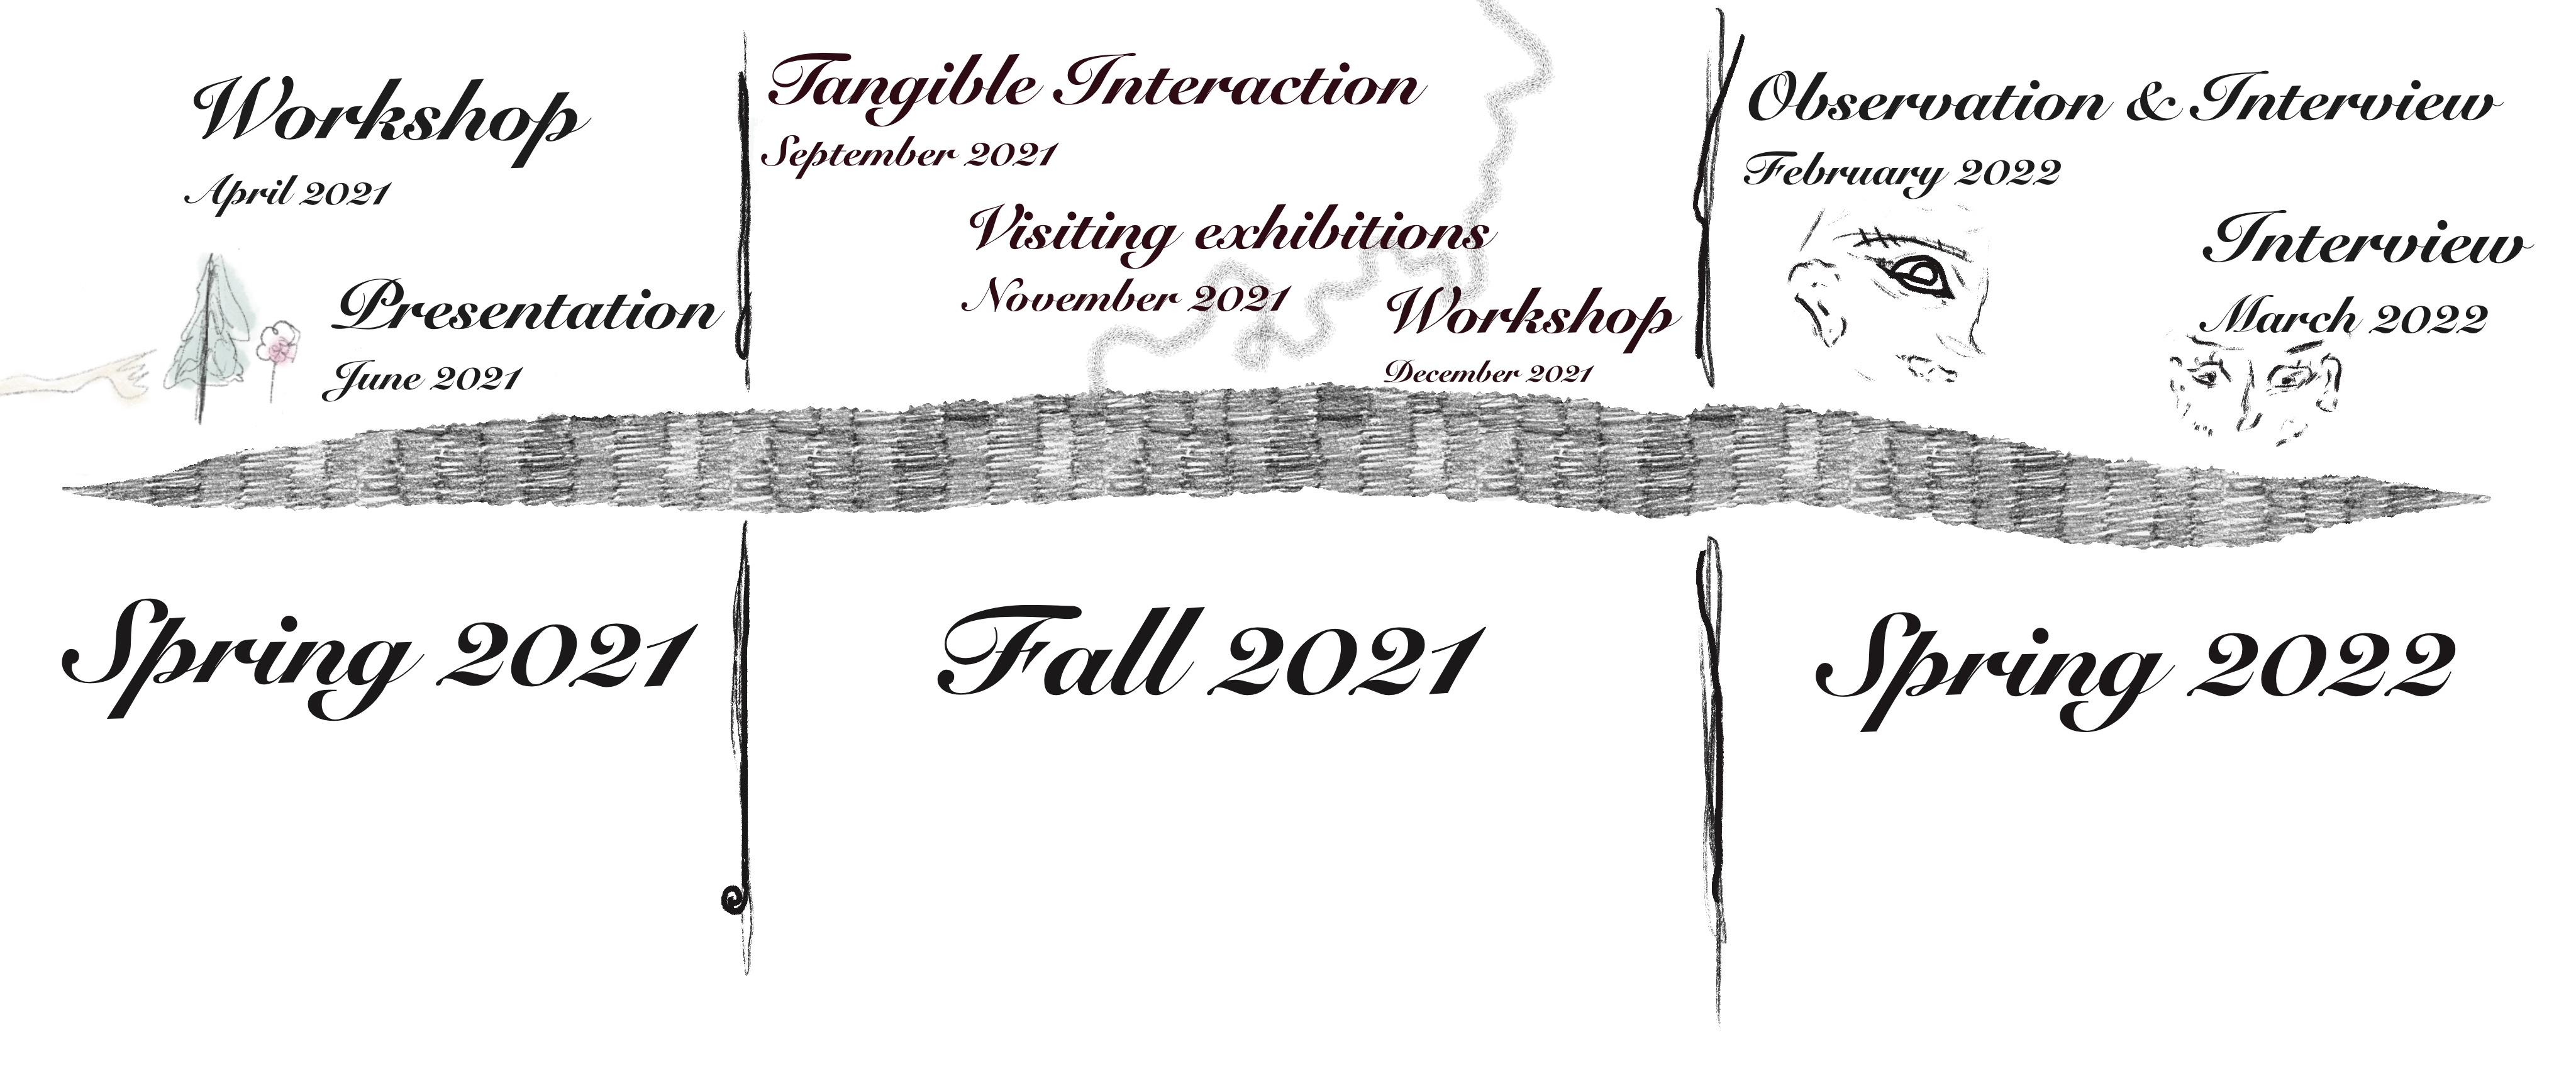
\includegraphics[width=14cm]{pictures/methodology/timeline.jpg}
\caption{Timeline of fieldwork}
\centering 
\end{figure}

The thesis project has lasted over the course of three semesters. From January to June spring of 2021, both theoretical and practical work was conducted. In January, we met our contact from Klimahuset and had our first viewing and walk-through of the museum's exhibition. Some weeks later, we were asked to host a workshop of our choosing that would take place in April. In February, we started a literature review focused on getting to know the museum domain and did so by reading critical literature on: exhibition practice \autocite{Thi_book}, narrative theories and learning in contemporary art museums \autocite{narrative_sitzia}, and on the subject of cultural analysis in museums \autocite{Miekebal_book}, as is evident in chapter 2: The Modern Museum and Sustainability. To explore the sustainability aspects of the current RQ (\emph{Interactive and visual installations addressing sustainability}), I worked conceptually and explored the topic; a distanced relationship to nature. This later manifested itself in the low-fidelity prototype that was presented at Klimahuset in June 2021; see section 8.3 in Chapter 8: Design Process.

All this work contributed to narrowing down the research area of interest and formulating a new research question. 

Next semester, August to December fall 2021, is where most practical research efforts were done. In September, we participated in a course about Tangible Interaction. Through this course, we were a part of a team who conceptualized, designed, and exhibited an interactive installation during the course duration of one month. Then came November, when we decided to visit different museums that exhibited interactive installations to experience, observe and collect data on different installations. In late December 2021, the Tangible Interaction group I was a part of was requested to exhibit our installation for a group of first-year master's students interested in writing about energy visualization. And then comes Spring 2022, where the main focus is writing up the thesis. In February, we were given the opportunity to observe two school classes in Klimahuset and given a little time to interview the working Docents - which we accepted. In March, our supervisor reached out to the newly opened MUNCH museum and presented us with the opportunity to interview a concept developer working there.

\begin{table}[h]
\centering
\begin{tabular}{| l | l|}
\hline
\textbf{Month} & \textbf{Event}\\
\hline
Jan. 21 & Initial contact and visiting Klimahuset for the first time \\
Feb. 21 & Started literature review on museums \\
Apr. 21 & Hosted a workshop with members of staff from Klimahuset \\
May 21 & Prototyped low-fid installation exploring input through plants \\
Jun. 21 & Held a presentation w/ prototypes at Klimahuset \\
Sep. 21 & Tangible Interaction course: designed an installation \\
Nov. 21 & Visited 5 interactive exhibitions \\
Dec. 21 & Held an energy visualisation workshop with Qi-installation \\
Feb. 22 & Observation of two school children classes in Klimahuset \\
Feb. 22 & Interview with two of Klimahuset's Docents \\
Mar. 22 & Interview w/ concept developer at Munch Museum \\
Apr. 22 & Analysis workshop sessions \\
May 22 & Visited one more interactive exhibition \\
\hline
\end{tabular}
\caption{Table of events}
\label{tab:abc}
\end{table}






\section{How the thesis have developed over time}
To describe and make clear how the thesis have developed over time, I will use \autocite{zimmerman_research_2014} model for interaction designers to carry out an RtD research project, and \autocite[]{zimmerman_discovering_2004} opportunity map to further describe how the design activities have produced knowledge during the research process.

To carry out an RtD research project, \autocite[]{zimmerman_research_2014} propose a team to follow five steps;
\begin{itemize}
    \item 1. Select
    \item 2. Design
    \item 3. Evaluate
    \item 4. Reflect and Disseminate
    \item 5. Repeat
\end{itemize}


\emph{Select} involves choosing a research problem or design opportunity worthy of investigation, and consider whether the research problem lends itself to investigation via RtD \autocite[p. 185]{zimmerman_research_2014}. \emph{Design} involves the beginning of design activities, ranging from literature review to understand the state of the art, conducting fieldwork, holding a design workshop, playing with a new material or by exploring ideas in the studio \autocite[p. 185]{zimmerman_research_2014}. Throughout the process of making and critiquing, the team should \emph{evaluate} and continually challenge their initial framing, while documenting the design moves and rationale for these moves, in addition to reflect on how the framing of the situation evolves and work to capture the reasons their framing changes \autocite[p. 185]{zimmerman_research_2014}.


Write out how the project fits into Zimmerman steps/ phases.

\section{Model of interaction design research}
Throughout this thesis project, there has been a major directional shift that has affected the research outcome - something which happened right about in the middle of things. I started this thesis project with a pretty clear goal to prototype and design an installation, but have ended up with a critical study of a number of interactive exhibitions and installations that I analyse to identify meaningful relationships or qualities in a museum space. To better show and talk-through this shift, I will use Fallman's model of interaction design research, which I often refer to as 'the design triangle', to better describe how my researching lens have shifted throughout and during the thesis project. It is also a means to explain as to why and how this thesis is fitted and give back to the interaction design research field.

As a design discipline, interaction design’s core can be found in an orientation towards the shaping of digital artefact, products, services, and spaces - with particular attention paid to the qualities of the user experience \autocite[p. 4]{fallman_triangle_2008}. In Fallman’s use of the model, the most interesting and rewarding results in interaction design research come not from taking a specific position in the model, but rather from moving or drifting in between different positions. Thus, as Fallman describe it, "moving in between different positions in the model is, more than anything else, a change of perspective" \autocite[p. 10]{fallman_triangle_2008}.


\begin{figure}[H]
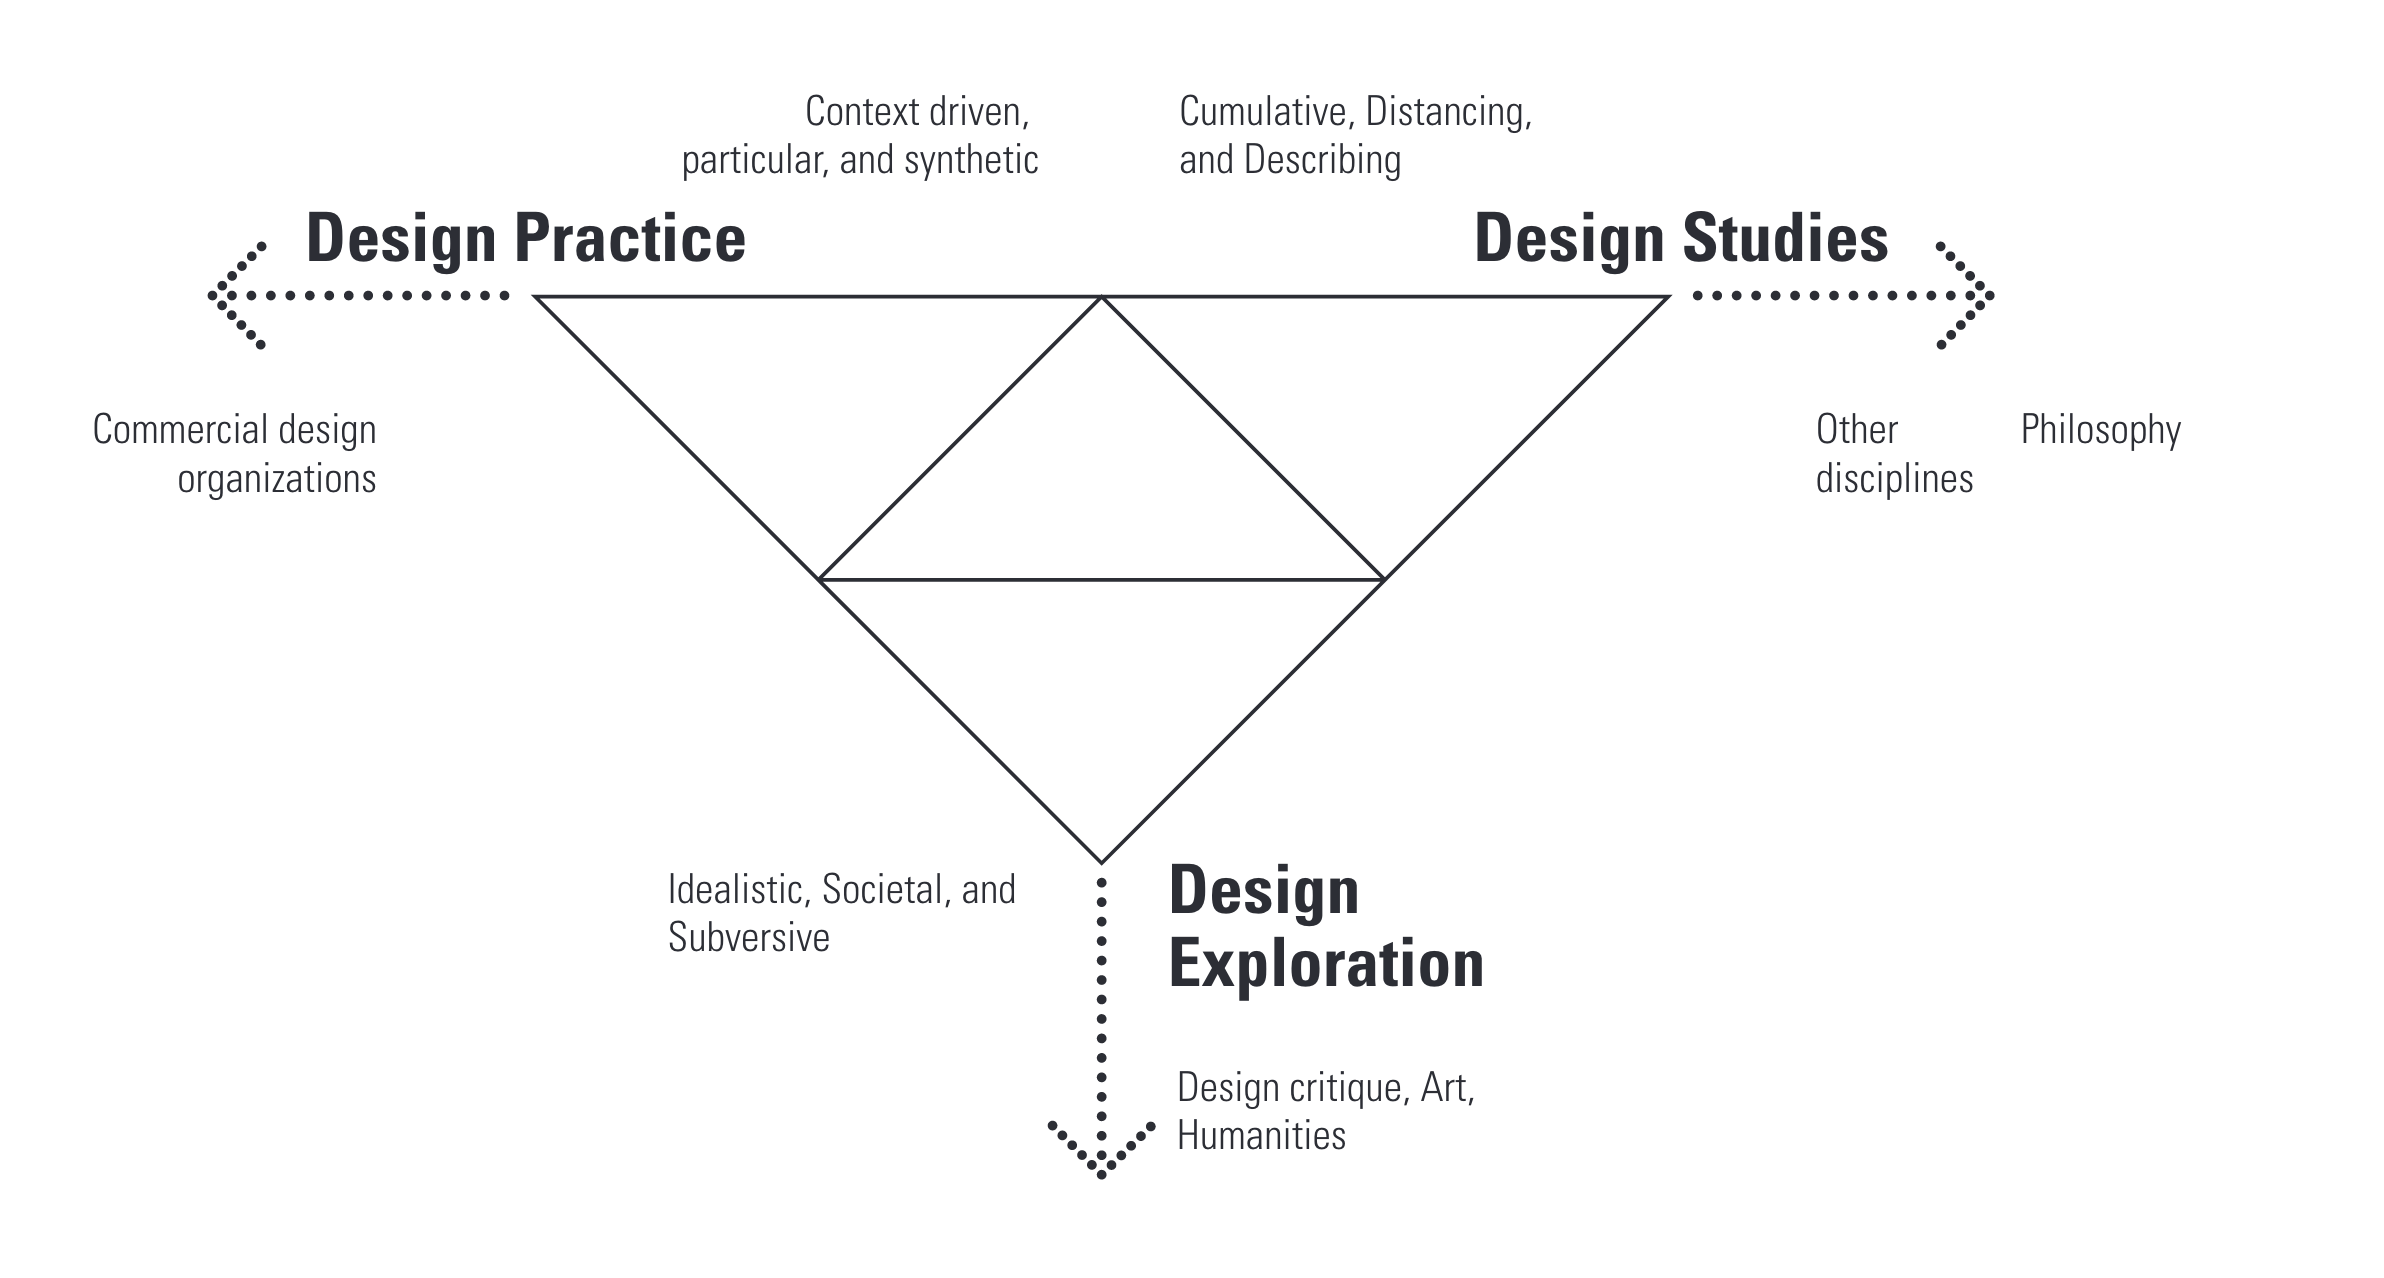
\includegraphics[width=13cm]{pictures/process/triangle.png}
\caption{"The model of interaction design research in its most basic form."}
\autocite[p. 5]{fallman_triangle_2008}
\centering 
\end{figure}

% In terms of doing research through design as a method for interaction design, Zimmerman et. al, explains that what is unique to research though design as an approach, is that it sees the design artefacts as outcomes that can transform the world from its current state to preferred state, which aligns with the domain problems I have accounted for in section 2.0, to address sustainability issues for a more sustainable future. Zimmermann et. al. further explain how the artefacts produced in this type of research become design examples, providing an appropriate channel for research findings to easily transfer to the HCI research and practise communities(Zimmermann et. al, p. 1, 2007).


Design study entails making space for reflections in some kind of structured way on one’s activities: organising reading circles and seminars; and opening up arenas for theoretical, methodological, and philosophical discussions to take place \autocite[p. 18]{fallman_triangle_2008}. The way I have gone forward with this, is to read up on museum practise as evident in chapter 1: Museums, as well as on the topic of sustainability, linking the museum practise up against sustainability. Specifically looking at how sustainability represents a contemporary discourse, and discussing this in relation to how museums want to address and disseminate more contemporary issues to stay relevant. 


\section{Table of datagathering that is not observations of installations}

\begin{table}[h]
\centering
\begin{tabular}{l | l| l}
\textbf{Type} & \textbf{Name} & \textbf{Museum}\\
\hline
Literature review & Museums and Sustainability & \\
Prototyping & The relationship between human and nature \\
Presentation & Exploring input through plants & Klimahuset\\
Exhibition & Liquid Life & Kistefoss \\
Observation & Climate Dialogue w/ 2 school classes & Klimahuset\\
Interview & Concept Developer & MUNCH\\
\end{tabular}
\caption{Other fieldwork}
\label{tab:abc}
\end{table}


\section*{Research question evolution}
In my attempt to answer how one can design meaningful interactive experiences in a museum space that addresses sustainability, I have chosen to look into three theoretical frameworks that give the means to understand interactive artefacts dialogic qualities - as an answer to how museum spaces can look at their respective installations and judge whether or not they stimulate the visitor to dialogue (conversations). The hypothesis is that there lies value for the museum to judge whether or not their installations promote dialogue. 

\begin{figure}[H]
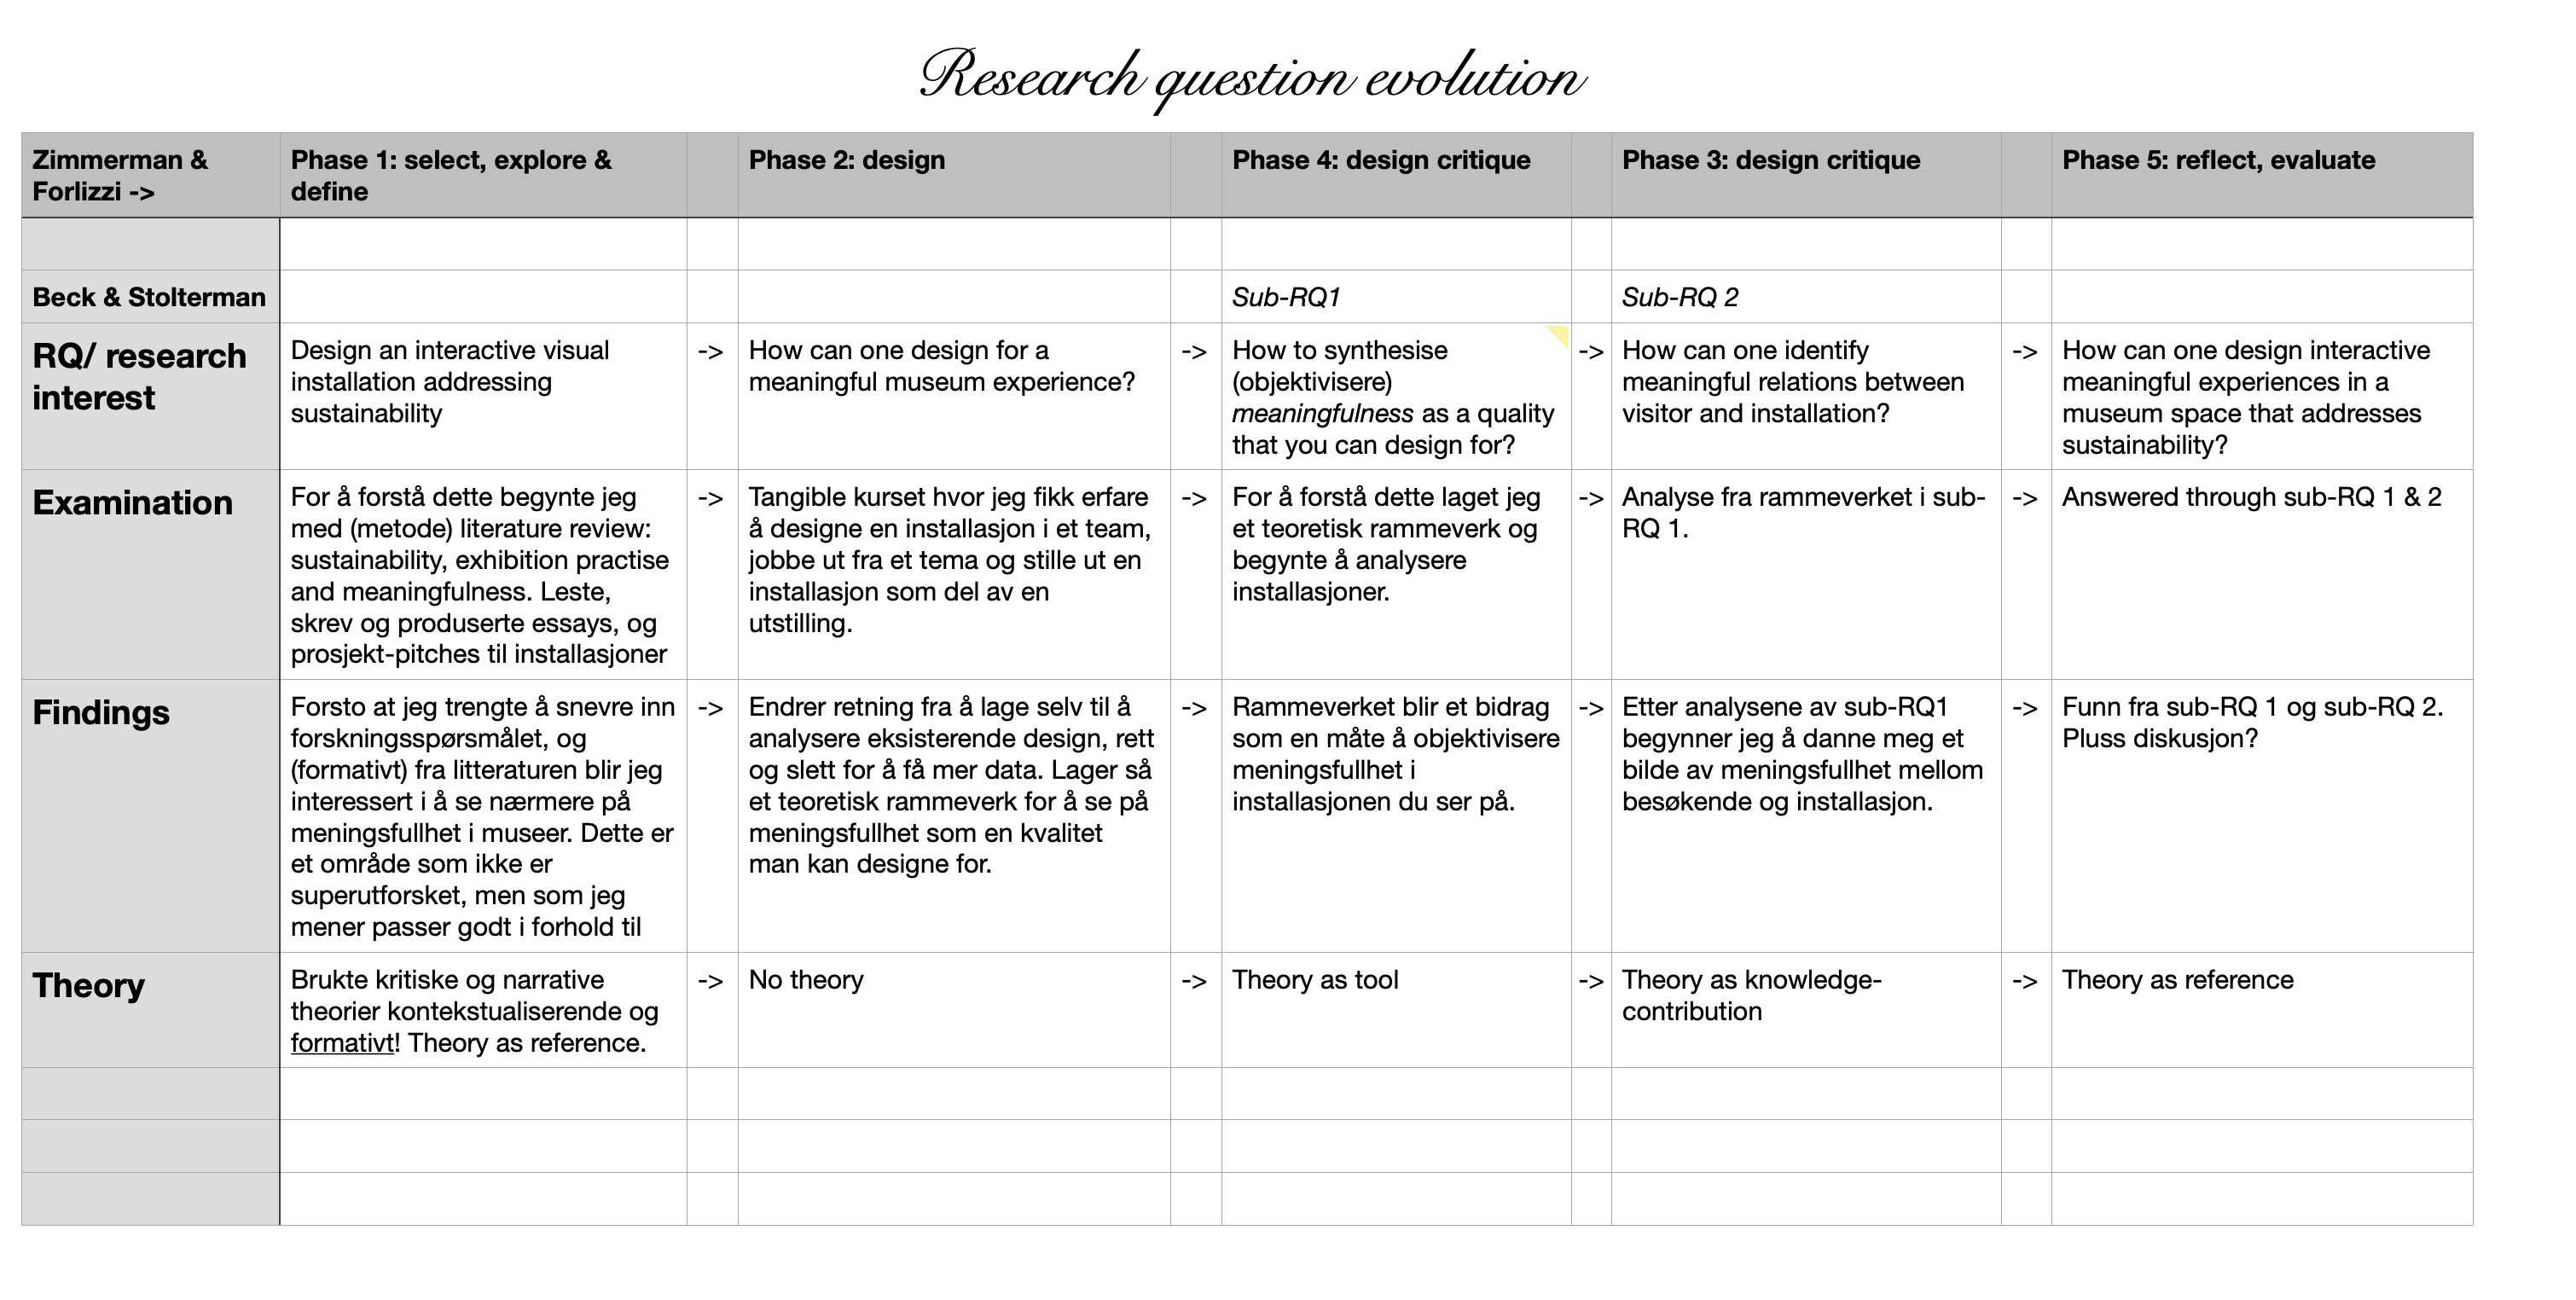
\includegraphics[width=21cm, angle=90]{pictures/process/rq_evolution.png}
\caption{Research question evolution}
\centering 
\end{figure}


\section{Generating knowledge through analysis of design}
The main intention of analysing existing interactive installations rather than designing, implementing, and evaluating one installation, has been to help inform the overarching research question. There have been discussions of whether researching through making artefacts intend to produce theory and what types of research outputs Research through Design can contribute to the different disciplines within HCI \autocite[p. 177]{zimmerman_research_2014}. The primary purpose of this thesis has been to contribute with knowledge that makes visible dialogic relations between interactive installations and visitor-experience in the museum space, to attempt to answer how one can design meaningful interactive experiences in a museum space. "By making different things intended to address the same problematic situation, RtD can reveal design patterns \autocite{Alexander_book} around problem framings, around specific interactions, and around how theory can be operationalized" \autocite[p. 178]{zimmerman_research_2014}.

I wanted to complement my theoretically informed framework for meaningfulness with learnings from the analysis of the design artefacts, to use the strengths of both theory and design to synthesise a solid framework.

\section{The role of prototyping in this thesis (unfinished)}

Research through design is a type of research practise where the researcher create artefact- or object prototypes to gain the necessary insight needed to drive and conduct the research project. Prototyping, or the use of prototypes can be used in a variety of ways, and in every stage throughout the project. In the field of human-computer interaction (HCI), software engineering and design, the term prototype is commonly used to signify a specific kind of object used in the design process \autocite[p. 2]{lim_anatomy_2008}. The prototypes are either physical or digital, and function as either a speculative solution, as a manifestation of a design idea, or to explore a design space - all in relation to the research scope and focus. Prototypes are the means by which designers organically and evolutionary learn, discover, generate and refine designs \autocite[p. 2]{lim_anatomy_2008}. They are design-thinking enablers deeply embedded and immersed in design practise, not just as tools for evaluating or proving successes or failures of design outcomes \autocite[p. 2]{lim_anatomy_2008}


In the search for a new way of thinking about prototypes and prototyping, based on the need for exploring and establishing a definition that differs from current approaches in software engineering contexts where engineers use prototypes to identify or satisfy requirements: Lim et. al., conceptualise prototypes as tools for traversing a design space where all possible design alternatives and their rationales can be explored \autocite[p. 2]{lim_anatomy_2008}. In that way, the prototype serves as a communicative manifestation, where the designer is enabled to communicate the rationales of their design decisions through the prototype \autocite[p. 2]{lim_anatomy_2008}. Prototypes stimulate reflections, and designers use them to frame, refine and discover possibilities in a design space \autocite[p. 2]{lim_anatomy_2008}. This new way of thinking about prototypes differs markedly from requirement-oriented approaches like software engineering, recognising design activities as flexible rather than rigid, reflective rather than prescriptive, and problem-setting rather than problem-solving (Schön, 1982). A design idea that satisfies all the identified requirements does not guarantee that it is the best design since a number of ways can meet each requirement \autocite[p. 2]{lim_anatomy_2008}. If the focus of prototyping is framing and exploring a design space, what matters is not identifying or satisfying requirements using prototypes but finding the manifestation that in its simplest form, filters the qualities in which designers are interested, without distorting the understanding of the whole \autocite[p. 2]{lim_anatomy_2008}. In order to support this perspective and to provide a stable foundation for the study of prototypes in HCI, Lim et. al. (2008) proposes a framework for conceptualising prototypes. The framework is an attempt to create an understanding of the nature of prototypes in general and to provide a language for articulating the characteristics of a particular prototype \autocite[p. 3]{lim_anatomy_2008}. Two fundamental aspects of prototyping form the basis of the framework:

1) prototypes are for traversing a design space, leading to the creation of meaningful knowledge about the final design as envisioned in the process of design, and
2) prototypes are purposefully formed manifestations of design ideas.
\autocite[p. 3]{lim_anatomy_2008}

Will answer these:
What values are important in my context?
What is my design outcomes?
What is my design space?
Experience prototyping? Am I going to prototype an experience?
Why and how do I intend a particular prototype to support the design process?



